\chapter{Theory}
\label{cha:theory}

Theories used in this study are presented here. They include software
development methodology, software metrics, reactive systems and some general
information regarding the \textit{libuv} library.

\section{Internet of Things}

The Internet of Things (IoT) is a relatively new paradigm of the internet where
not only people are interconnected, but \textit{everything} is. The term was
first heard in 1999 in a presentation by Kevin Ashton \cite{ashton2011internet}
and the popularity has since blossomed \cite{gubbi2013internet}. IoT can be
conceptualized as context-aware \textit{things} communicating with each other
and human-centered applications. The enabling applications are vast and include
domains from many areas of society - transportation, healthcare, homes, offices
and social domains to name a few. A good example is electricity consumption
control in homes. Electricity prices can be monitored and utilities such as
washing machines and heating can be optimized and only used when prices are low
\cite{atzori2010internet}. IoT can typically be explained as "one paradigm with
many visions" \cite{atzori2010internet} as there is no official definition of
the term. IoT is more than ubiquitous computing, embedded devices and
applications. It should not only be accessible by a small group of stakeholders
but embedded in today's open internet infrastructure. Referring to logistics an
IoT definition can be viewed as \textit{"[asking] for the right product in the
right quantity at the right time at the right place in the right condition and
at the right price"} \cite{uckelmann2011architectural}. Uckelmann et. al.
discusses these approaches and defines IoT as:

\begin{center}
\textit{"Internet of Things links
uniquely identifiable things to their virtual representations in the Internet
containing or linking to additional information on their identity, status,
location or any other business, social or privately relevant information at a
financial or non-financial pay-off that exceeds the efforts of information
provisioning and offers information access to non-predefined participants. The
provided accurate and appropriate information may be accessed in the right
quantity and condition, at the right time and place at the right price. The
Internet of Things is not synonymous with ubiquitous / pervasive computing, the
Internet Protocol (IP), communication technology, embedded devices, its
applications, the Internet of People or the Intranet / Extranet of Things, yet
it combines aspects and technologies of all of these approaches."}
\cite{uckelmann2011architectural}.
\end{center}

\subsection{Enabling technologies and challenges}

The state-of-the-art technologies used today in the IoT context include
sensoring equipment and networks such as the \textit{Radio Frequency
Identification} (RFID) and the \textit{Wireless Sensor Network} (WSN),
communication techniques like the \textit{IPv6 over Low-Power Wireless Personal
Area Network} (6LoWPAN) and \textit{Representational State Transfer} (REST) and
architectural approaches like \textit{middleware} and \textit{gateways}.

The RFID is a technique used to identify an object by letting a reader generate
an electromagnetic wave which in turn generates a current in a microchip that
transmits a code back to the reader. The code, also known as an
\textit{Electronic Product Code} (EPC), can be used to identify the object. EPC
is developed by EPCglobal, a global non-profit organization, with the purpose
to spread the use of RFID and create global standards for modern businesses
\cite{atzori2010internet}. An RFID tag can be passive, i.e. work without
battery power, or active, i.e. work with battery power. It basically consists
of an antenna, a microchip attached to the antenna and some form of
encapsulation. They vary in size and shape; from centimeter long 3D-shaped
capsules to 2D-shaped stickers. The fact that they can work without a battery,
meaning they theoretically can work forever, make them very practical to use in
different environments. \cite{want2006introduction}

In a survey from 2001, Akyildiz et. al.  \cite{akyildiz2002wireless} presents a
\textit{Wireless Sensor Network} containing hardware nodes capable of
monitoring its environment and transmit the received data to a server or host
acting as a sink. The sensor could be one of many types and be able to measure
temperature, humidity, movement, lightning condition, noise levels etc. This
leads into one of the major challenges in IoT: communication and networking.
Following the semantical meaning of IoT, which states \textit{"[it is] a world
wide network of interconnected objects uniquely addressable, based on standard
communication protocols"} \cite{bassi2008internet}, it is clear that every node
will produce its own content and should be retrievable regardless of location.
This puts pressure on the identification methods and the overall network
infrastructure for IoT. As remaining unused IPv4 addresses are closing in to
zero, the IPv6 protocol can be a natural next step for IoT devices to use
\cite{atzori2010internet}. 4 bytes are used to address devices in IPv4, wich
means the protocol can support around 4 billion devices. IPv6 on the other hand
use 16 bytes to address devices, meaning around $10^{38}$ devices can be
uniquely addressed.

6LoWPAN is a wireless technology suitable for resource-constrained nodes in the
IoT network. It is designed for small packet sizes, low bandwidth, low power
and low cost. It assumes a large amount of nodes will be deployed and that they
can be unreliable in terms of radio connectivity and power drain, thus making
this technology a good choice for wireless sensor nodes. \cite{kushalnagar2007ipv6}

%% Write stuff about REST

\subsection{Gateways}

A big challenge in IoT is, as described earlier, to connect every single device
to the internet. As for example devices in a WSN are deployed they do not
necessarily have the power and capacity to directly communicate to the
internet. A common approach to solve this problem is to add a gateway between
the devices and the internet, acting as an amplifier for the transmissions from
the devices \cite{zhu2010iot}. Chen et. al. \cite{chen2011brief} describes three
layers of domains in the IoT architecture: the \textit{sensing domain}, the
\textit{network domain} and the \textit{application domain}. The sensing domain
is where the primitive communication between the actual devices in the network
happen; for instance RFID and 6LoWPAN. This domain is layered under the network
domain and each piece of information sent from the sensing domain is
aggregated, filtered and wrapped in the network domain before being sent to the
application domain. Note that the information protocols used between the
sensing- and network domain and the network- and application domain does not
necessarily match. As some protocols are more suited for resource-constrained
devices, they might require modification to be able to communicate with more
standardized protocols, like the \textit{Internet Protocol} (IP). E.g. the EPC
code generated by the RFID can not be put on an IP stack as is, but it could be
mapped to an IPv6 address via a gateway and thereby be identified and usable
through the internet \cite{lee2007epc}.

The gateways reside in the network domain. They act as a bridge between the
devices and the internet. The approaches towards implementing IoT gateways vary

%% Should list different approaches in the industry, from large companies to
%% smaller projects.

\section{Software development methodology}

There exists a numerous amount of ways to develop software. In plan-based
methodologies, including the \textit{waterfall model}, the way of working is
highly inspired by traditional engineering such as manufacturing and
construction. Given a set of phases in the development, each phase must be done
before the next phase starts. These phases include \textit{requirement
definition}, \textit{design}, \textit{implementation}, \textit{testing} and
\textit{release} \cite{crookshanks2014practical}. On the other end of the
spectra lies the \textit{agile} methodologies. Initially developed as a
response to the frustration of the static, slow-going process of the well-used
waterfall model, it is based on the understanding that software requirements
are highly dynamic and most certainly change over time
\cite{moniruzzaman2013comparative}.

Vijayasarathy and Butler \cite{vijayasarathy2016choice} found in an online
survey they conducted in 2016 that around a third of all software projects were
using the waterfall model as main software methodology. Following were the
agile methodologies \textit{Agile Unified Process} and \textit{Scrum}. They
also found that multiple methodologies were often used in the same project.
For instance the agile method \textit{Joint Application Development} was used
in one project to identify requirements, while the waterfall model was used in
the remainder of the project.

\subsection{Scrum}

Scrum is an agile framework utilized by small teams to develop simple and
complex products. Scrum is not only used to do software development, it can be
applied to any development - even a book \cite{sims2012scrum}. In Scrum there
are three main components: \textit{roles}, \textit{artifacts} and \textit{the
sprint cycle}. Roles are taken by people in the team, artifacts are tools used
by the team and the fundamental pulse of the project is the sprint cycle. Three
distinct roles are recognized: \textit{product owner}, \textit{Scrum master}
and \textit{team member}. The product owner is the team's representation of the
\textit{stakeholders} of the product (mainly the business related
stakeholders). He is responsible for making the team always do most valuable
work, he holds the vision of the product, he owns the \textit{product backlog}
and creates acceptance criteria for the backlog items. The scrum master is the
team's coach guiding them to become a high-performing, self-organizing team. He
helps the team apply and shape the agile practices to the team's advantage. A
team member is responsible for completing \textit{user stories}, create
\textit{estimates} and decides what tools to use in the upcoming
\textit{sprint}. \cite{sims2012scrum}

The artifacts recognized by Scrum are called \textit{product backlog},
\textit{sprint backlog}, \textit{burn down charts} and \textit{task board}. The
product backlog consists of a list deliverables that can be anything of value
for the product, e.g. features and documentation changes. Items in the list are
also called \textit{user stories} and they are ordered by priority. They
include information such as who the story is for, what needs to be built, how
much work is needed to implement it and what the acceptance criteria is. Prior
to a \textit{sprint} user stories are derived into practical \textit{tasks}
usually performed by a single team member. The sprint backlog is populated by
these tasks and they are expected to be finished within the time limit of the
sprint. To monitor the status of the sprint or the entire project, the burn
down chart is used. It is a diagram showing how much work is left to be done.
The Y-axis shows the amount of tasks and the X-axis the time. As time progress
the amount of tasks are hopefully decreasing. The task board is used to help
the team inspect their current situation. It usually consists of three columns:
\textit{To do}, \textit{Doing} and \textit{Done}. Each column consists of tasks
(or symbols of tasks) in the current sprint, and gives the team a visual on
what tasks are yet to be done. \cite{sims2012scrum}

A Scrum project is split into a series of sprints. They are time limited
smaller versions of the entire project where a pre-defined amount of tasks are
to be completed within the sprint. When a sprint is finished a potentially
working product is demonstrated. The benefit of short-lived sprints is that the
team receives frequent feedback on their work, giving them a better presumption
to improve future sprints. From a business perspective, the sprint method
provides greater freedom to decide if a product should be shipped or further
developed. A sprint consists of a number of meetings: \textit{sprint planning},
\textit{daily Scrum}, \textit{story time}, \textit{sprint review} and
\textit{retrospective}. A sprint always starts with a sprint planning. It is a
meeting where the product owner and the team decides which user stories will be
a part of the sprint backlog in the upcoming sprint. This is also where the
team derive the user stories into tasks. Every day the team also has brief
daily Scrum meetings. Each team member shares what tasks they completed since
the previous meeting, what tasks they expect to complete before the next and
what difficulties they are currently facing. Every week, during story time, the
product backlog is again reviewed by the team and the product owner. This time
each user story is evaluated to refine its acceptance criteria. If there are
large stories in the backlog they are also split into smaller stories to make
them easier to understand and easier to complete within a sprint. The sprint
review marks the public end of the sprint. Here the completed user stories are
demonstrated to the stakeholders and feedback is received. After this meeting
the team has a retrospective meeting where they discuss what strategy changes
can be made to improve the next sprint. \cite{sims2012scrum}

\section{Reactive systems}

Systems required to continually respond to its environment are called
\textit{reactive} systems. Harel and Pnueli \cite{harel1985development}
elaborates on different system dichotomies, for instance deterministic and
nondeterministic systems. Deterministic systems have unique actions which
always generates the same output. Nondeterministic systems do not have that
property and it can cause them to be more difficult to handle. Another
dichotomy is sequential and concurrent systems. Concurrent systems cause
problems which are easily avoidable in sequential ones. For instance the mutual
exclusion problem where it is not always trivial what process owns what
resource and whether it is safe to modify a resource that can be used by
another process. A more fundamental dichotomy is presented by Harel and Pnueli:
\textit{transformational} and \textit{reactive} systems. A transformational
system transforms its input and creates new output. It can continually prompt
for new input. A reactive system is prompted the other way around: from the
outside. It does not necessarily compute any input, but it maintains a
relationship with its outside environment. A reactive system can be
deterministic or nondeterministic, sequential or concurrent, thus making the
transformational/reactive system dichotomy a fundamental system paradigm.
\cite{harel1985development}

\subsection{Specifications for reactive systems}

Harel and Pnueli \cite{harel1985development} presents a method for decomposing
complex system using \textit{statecharts}. Drawn from the theories of
\textit{finite state automata}, a system can be expressed using states. This is
particularily useful for reactive systems that can react to a large amount of
different inputs. One powerful feature with statecharts is its ability to
handle hierarchical states. If a system has a numerous amount of input
combinations, a large set of states must be created which in the long run is
not appropiate in terms of scalability. One solution to this is hierarchical
states in which a state can hold a number of other states. Fundamentally, a
state undergo a transition to another state when an action is performed on that
state. \cite{harel1985development}

Ardis et al \cite{ardis1996framework} created a specification for a telephone
switching system which later was tested on a number of languages. They started
by describing some general properties of the system in a list. In general, the
list had the format:

\begin{enumerate}
\item
  When event $X_1$ occurs,
\begin{enumerate}
\item
  If some condition or property of the system holds true, call action $Y_1$
\item
  Otherwise, call action $Z_1$
\end{enumerate}

\item
  When event $X_2$ occurs,
\begin{enumerate}
\item
  Call action $Y_2$
\end{enumerate}

\item
  And so on...
\end{enumerate}

They then implemented a system fullfilling the requirements in a set of
different languages. Most languages fit well for reactive systems since their
semantic allows and makes it easy to build and define different state machines.
They also did one implementation in C in which they had two solutions: one
using arrays to hold all the different actions and states and one using
switch-blocks.

However, specification of primitive components can still be a challenge.
Non-trivial steps might be required to transition from one state to another.
Hummel and Thyssen \cite{hummel2009behavioral} presents a formal method to
specify a reactive system using stream based I/O-tables. In addition to
generating a simple and understandable description of the system, the method
helps formalize inconsistent requirements.

\section{Choosing programming language for embedded systems}

In embedded systems programming, both hardware and software is important. Nahas
and Maaita \cite{nahas2012choosing} mentiones a few factors to be considered
when choosing a programming language for an embedded system:

\begin{itemize}
\item
  The language must take the resource constraints of an embedded processor
  into account
\item
  It must allow low-level access to the hardware
\item
  It must be able to re-use code components in the form of libraries from other
    projects
\item
  It must be a widely used language with good access to documentation and other
    skilled programmers
\end{itemize}

There is no scientific method for selecting an appropiate language for a
specific project. Selection mostly relies on experience and subjective
assessment from developers. It was however shown in 2006 that over 50 \% of
embedded system projects were developed in C and 30 \% were developed in C++.
Barr \cite{barr1999programming} states that the key advantage of C is that it
allows the developer to access hardware without loosing the benefits of
high-level programming. Compared to C, C++ offer a better object-oriented
programming style but can on the other hand be less efficient.
\cite{nahas2012choosing}

\section{libuv}

libuv is an asynchronous I/O cross-platform library written in C. It is one of
the major core systems of Node.js, a popular JavaScript runtime engine. libuv's
central part is the single-threaded event loop which contains all I/O
operations. The event loop notifies any I/O events in a callback fashion using
abstractions called \textit{handles} and \textit{requests}. Handles are
long-lived structures and are operated on using requests. Requests usually only
represent one I/O operation on a handle. Each I/O operation performed on the
event loop is \textit{non-blocking}, meaning they instantly return and
abstracts away any concurrency necessary. To handle network I/O libuv make use
of platform specific functionality, such as \textit{epoll} for Linux. For file
I/O libuv utilizes its \textit{thread pool} to make the operation non-blocking.
All loops can queue work in this thread pool making it ideal for external
services or systems that do not want to block any I/O. libuv include handles
for \textit{UDP} and \textit{TCP} sockets, file and file system, \textit{TTY},
timers and \textit{child processes}. \cite{libuv-docs}

\begin{figure}[h]
  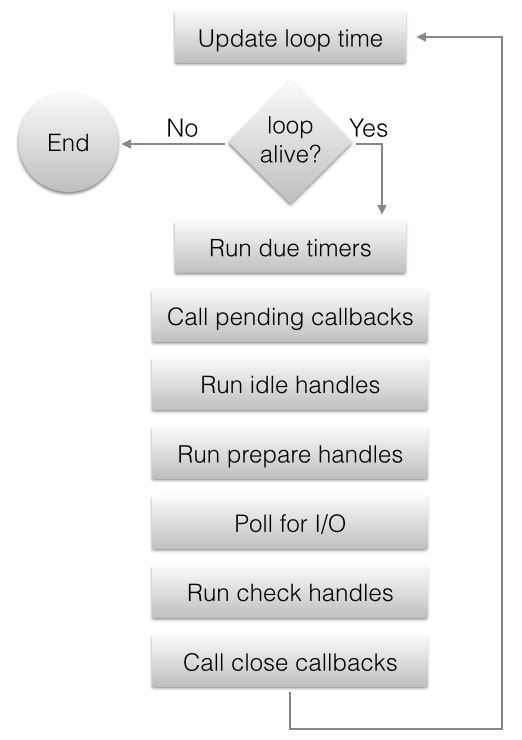
\includegraphics[width=7cm]{loop_iteration}
  \centering
  \caption[libuv event loop]{The stages each event loop iteration step through
  in libuv \cite{github2017libuv-loop_iteration}.}
  \label{fig:loop_iteration}
\end{figure}

Figure \ref{fig:loop_iteration} demonstrates the stages each event loop
iteration step through. A loop is considered to be alive if there are any
active handles or requests. For instance, if a TCP socket is closing its
connection the handle structure is freed from the heap and both the request and
handle are no longer active. If they were the last being active the loop dies.
The steps are described briefly: \cite{libuv-docs}

\begin{enumerate}
  \item The loop time is updated and stored for the entire iteration.
  \item If the loop is alive the iteration starts, otherwise it dies.
  \item All active timers who are scheduled to timeout have their callbacks
    called.
  \item Pending callbacks are called; they are I/O callbacks deferred from the previous
    iteration.
  \item Callbacks registered for idle handles are called. Idle handles are good
    for low priority activity.
  \item Callbacks that should be called right before polling for I/O can be
    registered with prepare handles, whose callbacks are called here.
  \item The time to poll for I/O is calculated here. It either blocks for 0
    seconds, the timeout for the closest timer or infinity. Depending on
    whether there are active idle handles or requests or if the loop is about
    to close, the time is 0. \label{item:poll_time_calculation}
  \item I/O is polled and the loop is blocked. All handles monitoring I/O will
    have their callbacks called.
  \item Callbacks that should be called right after polling for I/O can be
    registered with check handles, whose callbacks are called here.
  \item Handles being closed have their close callbacks called.
  \item If the loop was configured to only run once and no I/O callbacks were
    called after the poll, timers might be due since time could have elapsed
    during the poll. Those timers gets their callbacks called.
  \item Depending on the loop's configuration and if it is still alive, the
    loop exits or continue.
\end{enumerate}

The following example provided by Marathe \cite{uvbook} shows an idle handler
and its corresponding callback. As seen in Figure \ref{fig:loop_iteration} and
explained in step \ref{item:poll_time_calculation} idle handles and their
callbacks are called every iteration with 0 poll time.

\lstinputlisting[
  style=customc,
  caption={libuv example with an idle handle \cite{uvbook}.},
  label={listing:idle_handle}
]{figures/libuv_idle_handle_example.c}

libuv includes a number of data types and functions which can be found in its
documentation \cite{libuv-docs}.

\section{Software metrics}

In all engineering fields, measurement is important. Measuring software is a
way for an engineer to assess its quality and a large number of software
metrics have been derived during the years \cite{aggarwal2006empirical}.

Previous research show that software process improvements is key for both large
and small successful companies. However, it requires a balance between formal
process and informal practice. Large companies tend to lean more towards the
formality of things and employees are given less space to be creative. On the
other hand, small companies tend to do the opposite: employees are given
freedom to explore solutions while formal processes are being put aside. Dybå
\cite{dybaa2003factors} suggests that "formal processes must be supplemented
with informal, inter-personal coordination about practice". It is also
important to note how failure is handled. Failure is essential for improving
learning and questioning the status quo inside both companies and software. If
failure is unacceptable, the organizational competance can decrease when facing
change in the environment. When a company is successful it will grow larger
with repeated success and there is no financial reason to change what already
works and generates revenue. However, eventually when the environment changes
there might be good reasons to dust off legacy systems and introduce some new
patches. The cost of doing so might depend on whether the system was initially
built with maintenability in mind. \cite{dybaa2003factors}

\subsection{Maintainability}

Maintainability can be measured in many ways. Aggarwal et al.
\cite{aggarwal2006empirical} suggests that some metric results can be derived
from others. In the same way the area and diagonal can be derived from the
width and height of a table, some metrics may provide redundant information.
Oman and Hagemeister \cite{oman1992metrics} proposes a quantitative approach
where multiple metrics can be combined into a unified value. Software
maintainability can be divided into three broad categories:

\begin{itemize}
\item The management practices being employed
\item Hardware and software environments involved in the target software system
\item The target software system
\end{itemize}

Oman and Hagemeister further derive the target software system into additional
categories:

\begin{itemize}
\item Maturity attributes
\item Source code
\item Supporting Documentation
\end{itemize}

Maturity attributes include metrics such as the \textit{age} of the software
since release, \textit{size} in terms of non-commented source statements and
\textit{reliability} which can be measured as the rate of failures per hour.
Source code include metrics on how the software is decomposed into algorithms
and how they are implemented, e.g. the number of modules and the cyclomatic
complexity averaged over all modules. It also includes metrics on the
information flow in the system, e.g. the number of global data types and
structures, the number of data structures whose type is converted and the
number of lines of code dedicated to I/O. Coding style metrics are also
included, e.g. the percentage of uncrowded statements (only one statement per
line), the number of blank lines and the number of commented lines are taken
into account. Supporting documentation are evaluated in a subjective manner.
Metrics include traceability to and from code implementation, verifiability of
the implementation and consistency of the writing style and comprehensibility
of the document. \cite{oman1992metrics}

To assess these metrics, Oman and Hagemeister introduces a formula:

$$
\prod_{i=1}^m{W_D_i(\frac{\sum_{j=1}^n{W_A_jM_A_j}}{n})_i}
$$

where $W_D_i$ is the weight of influence of software maintainability category
$D_i$, e.g.  source code control structure. $W_A_j$ is the weight of influence
of maintainability attribute $A_j$, e.g. software age. $M_A_j$ is the measure
of maintainability attribute $A_j$. The values should be structured so that
they range from 0 to 1, thereby showing a percentage of their correctness.
Worth noting is that not all attributes have to be measured, only those of
significant value.

\subsection{Measuring maintainability in C++}

Some metrics might not be suitable for object-oriented (OO) languages and C++
in particular. Wilde and Huitt \cite{wilde1991maintenance} studies some of the
main difficulties regarding maintenance as in "post deployment support" of
OO-languages. These languages introduces the concepts of \textit{object class
inheritance hierarchy} and \textit{polymorphism} which in some sense helps give
programmers a better understanding of their programs, but the maintenance
burden will unlikely disappear completely. One issue with analyzing OO source
code is \textit{dynamic binding}. An object variable might not necessarily
refer to its declared class type, but it can also refer to any of its
descendants in the class hierarchy. This makes static analysis complicated,
e.g. it is not always known what implementation of a method will be used when
the method is called on an object.

Rajaraman and Lyu \cite{rajaraman1992reliability} have also studied the
shortcomings on some traditional maintainability metrics on OO-languages. For
instance, they look on the metric \textit{statement count} which can predict a
software's complexity. It is built on the assumption that "the more detail that
an entity possesses, the more difficult it is to understand"
\cite{rajaraman1992reliability}. The metric simply counts the number of
statements in a program or module. They criticize the metric for not taking the
program's context into account and that it is not easy to determine what
exactly a statement is. They also criticize McCabe's
\cite{mccabe1976complexity} \textit{cyclomatic complexity measure} that
calculates a program's complexity by taking the number of edges in a program
flow graph, the number of nodes and the number of connected components into
account (nodes are abstractions of sequential blocks of code and edges are
conditional branches in the program). The critique involves, as stated earlier
regarding statement count, that the metric ignores the context in the program
and has no support to take the complexity of each statement into account.

Rajaraman and Lyu \cite{rajaraman1992reliability} defines four measures of
\textit{coupling} in their paper. They define the term coupling as "[...] a
measure of association, whether by inheritance or otherwise, between classes in
a software product". Abstracting the program to a directed multigraph, each
node represents a class and each edge represents a reference from one node to
another through variable references and method calls. Two of the proposed
measures, \textit{Class Coupling} and \textit{Average Method Coupling} resulted
in highest correlation (though not statistically significant) with perceived
maintainability when tested on a number of C++ programs. Class Coupling for a
class $C$ is defined as the sum of each outgoing edge from $C$; i.e. the sum of
all global variable references, all global function uses, all calls to other
class methods and all local references to other class instances. Average Method
Coupling is a ratio number between a class $C$'s Class Coupling and its total
number of methods, i.e. $AMC = CC / n$ where $n$ is the total number of methods
declared in $C$.
